\setcounter{section}{0}
\section{Hình thành kiến thức mới}

\subsection{Mở đầu}
Từ buổi sơ khai của loài người, khi đi trong rừng thẳm hoặc lênh đênh trên một vùng biển rộng, trong điều kiện thiếu các công cụ để xác định lộ trình, bầu trời đã trở thành nơi duy nhất để con người có thể định hướng đích đến hay đơn giản là để trở về nhà. Trong trường hợp này, con người đã xác định phương hướng như thế nào?
\subsection{Hình thành kiến thức mới}
\subsubsection{Thiên cầu}
Thời cổ đại, con người quan niệm vũ trụ được giới hạn trong một hình cầu với Trái Đất nằm ở trung tâm. Các ngôi sao được cố định vào vòm cầu này, do đó chúng cách đều Trái Đất. Vòm trời hình cầu tưởng tượng này còn được gọi là thiên cầu.

Thiên cầu là một quả cầu giả định có bán kính rất lớn với tâm đặt ở Trái Đất. Các thiên thể và sự chuyển động của chúng được phản chiếu trên thiên cầu. Để xác định vị trí của các thiên thể trên bầu trời, ta gắn một hệ trục tọa độ vào thiên cầu:

\begin{minipage}[l]{0.6\textwidth}
	
	\begin{itemize}
		\item Gốc tọa độ O: vị trí của người quan sát thiên thể.
		\item Đường thẳng đứng đi qua đỉnh đầu người quan sát, cắt thiên cầu tại điểm Z trên đỉnh đầu và điểm Z' dưới chân người quan sát. Hai điểm Z và Z' đối xứng với nhau qua gốc tọa độ O và lần lượt được gọi là thiên đỉnh và thiên để.
		\item Nếu người quan sát đứng tại O nhìn về hướng Bắc (N) thì bên phải và trái người quan sát lần lượt là hướng Đông (E) và hướng Tây (W), phía sau người quan sát là hướng Nam (S). Qua bốn điểm N, W, S, E trên thiên cầu, ta vẽ được một vòng tròn lớn gọi là đường chân trời (vòng NESW).
		\item Vòng tròn lớn đi qua thiên đỉnh Z và thiên để Z', đồng thời vuông góc với đường chân trời gọi là vòng thẳng đứng.
	\end{itemize}
\end{minipage}
\begin{minipage}[r]{0.4\textwidth}
	\begin{center}
		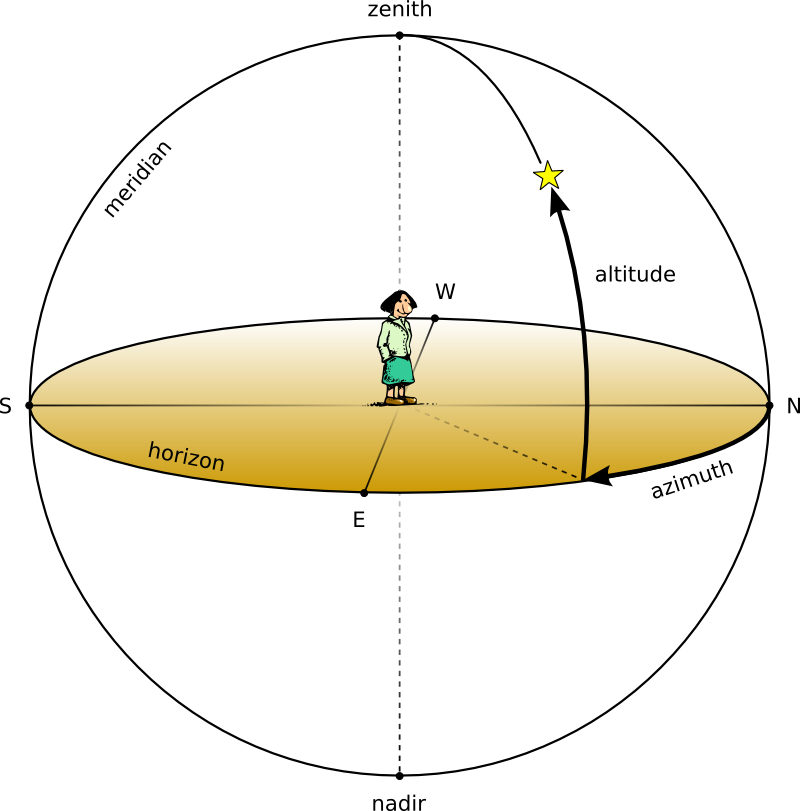
\includegraphics[scale=0.2]{../figs/G10-033-1.png}
	\end{center}
\end{minipage}

\subsubsection{Bản đồ sao - Các chòm sao trên nền trời}
Sao là những thiên thể khổng lồ nóng sáng, có khối lượng lớn. Mặt Trời là ngôi sao ở gần Trái Đất nhất.

\begin{minipage}[l]{0.6\textwidth}
	
	Khi các sao chuyển động, chúng sẽ phản chiếu lên mặt thiên cầu. Khi quan sát từ Trái Đất, ta thấy các sao luôn chuyển động trên bầu trời theo hướng từ Đông sang Tây với tốc độ khác nhau. Nhưng sao Bắc Cực ở gần cực Bắc của Trái Đất gần như không thay đổi vị trí.
	
	Dựa vào đặc điểm của các chòm sao vào thời điểm quan sát được, các nhà chiêm tinh đã tưởng tượng hình ảnh các chòm sao và gán cho chúng các tên gọi để nhận diện trên bầu trời.
	
	Để xác định được các chòm sao trên bầu trời, các nhà thiên văn đã lập bản đồ sao. Bản đồ sao gồm hình ảnh các chòm sao được định vị trên bầu trời dựa vào vị trí quan sát, thời điểm quan sát ở mặt đất theo các vĩ độ nơi quan sát.
	
\end{minipage}
\begin{minipage}[r]{0.4\textwidth}
	\begin{center}
		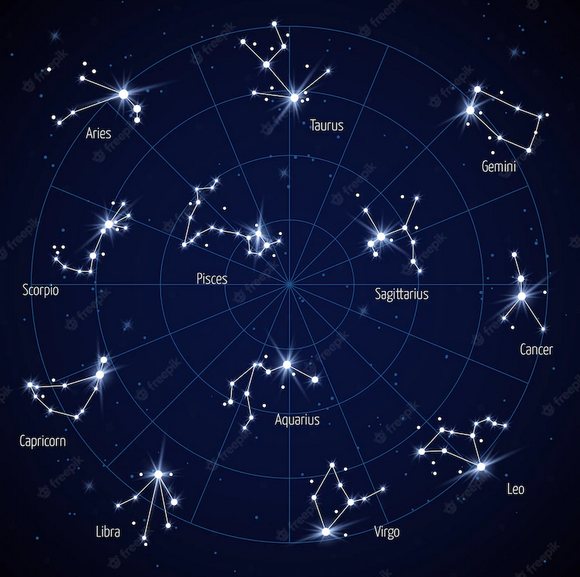
\includegraphics[scale=0.5]{../figs/G10-033-2.png}
	\end{center}
\end{minipage}

Để xác định phương hướng trên mặt đất, chỉ cần xác định được hướng Bắc tức là hướng đến thiên cực Bắc. Có một ngôi sao nằm rất gần thiên cực Bắc (cách thiên cực Bắc khoảng $1^\circ$) được gọi là sao Bắc Cực. Nó là sao sáng nhất trong chòm Gấu Nhỏ. Tuy nhiên, đây không phải là sao sáng nhất trên bầu trời đêm.

\begin{minipage}[l]{0.6\textwidth}
	Dựa vào chòm sao Gấu Lớn: Đầu tiên, ta xác định vị trí của chòm sao Gấu Lớn dựa vào bản đồ sao. Sau đó, ta xác định vị trí của hai ngôi sao sáng nhất của chòm sao này, là sao $\alpha$ và sao $\beta$. Ước lượng khoảng cách $d$ giữa hai sao $\alpha$ và $\beta$. Tiếp theo, ta vẽ đường tưởng tượng nối liền hai sao này và kéo dài theo hướng Bắc từ sao $\beta$ đến sao $\alpha$. Từ sao $\alpha$, ước lượng vị trí nằm ở khoảng cách $d'=5d$ dọc theo đường tưởng tượng vừa vẽ. Đó chính là vị trí của sao Bắc Cực.
	
	Dựa vào chòm sao Thiên Hậu: Vẽ đường tưởng tượng nối hai sao $\gamma$ và $\delta$, ước lượng khoảng cách $d$ giữa chúng. Từ sao $\gamma$, ta xác định vị trí của sao Bắc Cực tại điểm cách sao $\gamma$ một đoạn $d'=7d$ dọc theo đưởng tưởng tượng vuông góc với đường nối $\gamma - \delta$ cùng phía với sao $\epsilon$.
\end{minipage}
\begin{minipage}[r]{0.4\textwidth}
	\begin{center}
		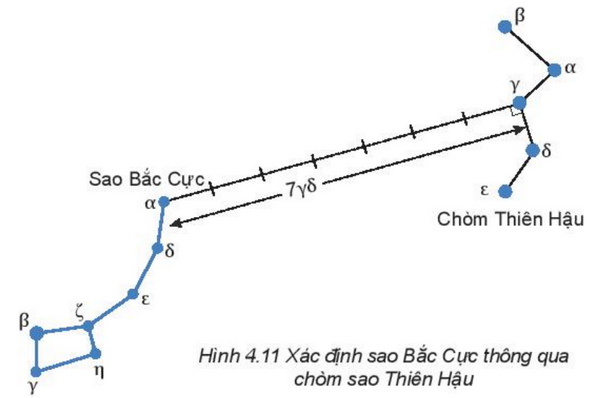
\includegraphics[scale=0.5]{../figs/G10-033-3.png}
	\end{center}
\end{minipage}

%\subsection{Mở rộng}
%\subsubsection{Lịch sử về sự phân chia Hoàng Đạo}
%Đai Hoàng Đạo là một khu vực của bầu trời kéo dài khoảng $8^\circ$ bắc hoặc nam (tính theo hệ tọa độ thiên văn) của Hoàng Đạo, đường đi rõ ràng của Mặt Trời trên khắp thiên cầu trong suốt năm.

%Trong chiêm tinh học phương Tây, đai Hoàng Đạo được chia thành mười hai cung hoàng đạo, mỗi cung chiếm $30^\circ$ của kinh độ thiên cầu và gần như tương ứng với các chòm sao Bạch Dương, Kim Ngưu, Song Tử, Cự Giải, Sư Tử, Xử Nữ, Thiên Bình, Thiên Yết, Nhân Mã, Ma Kết, Bảo Bình và Song Ngư.

%Mười hai cung chiêm tinh tạo thành một hệ tọa độ thiên thể, hay cụ thể hơn là một hệ tọa độ chiết trung, lấy Hoàng Đạo làm gốc của vĩ độ và vị trí của Mặt Trời tại điểm xích đạo là gốc của kinh độ.

%Sự phân chia của Hoàng Đạo thành các cung Hoàng Đạo bắt nguồn từ thiên văn học Babylon trong nửa đầu của Thiên niên kỷ 1 TCN.

%Vào khoảng cuối thế kỉ thứ 5 TCN, các nhà thiên văn học Babylon đã chia Hoàng Đạo thành mười hai cung bằng nhau. Theo tính toán của vật lí thiên văn hiện đại, đai Hoàng Đạo được giới thiệu trong khoảng từ năm 409 đến 398 TCN.
%\subsubsection{Mười hai cung Hoàng Đạo}
%Điểm khởi đầu theo lý thuyết của cung Bạch Dương là xuân phân. Các cung khác cứ thế nối tiếp. Từ năm 1797 đến năm 2043, ngày xuân phân (theo giờ UT - Universal Time) luôn rơi vào ngày 20 hoặc 21 tháng 3.

%Các nhà thiên văn học Babylon đã cố định đai Hoàng Đạo liên quan đến các ngôi sao, khởi đầu của Cự Giải ở cuối "Ngôi sao sinh đôi" (Pollux) và sự khởi đầu của Bảo Bình tại phía sau "Ngôi sao con dê" ($\delta$ Capricorni). Các kiểu phân chia này không tương ứng chính xác với nơi các chòm sao bắt đầu và kết thúc trên bầu trời; điều này sẽ dẫn đến một sự phân chia bất thường. Mặt Trời trên thực tế đã đi qua ít nhất 13, chứ không phải 12 chòm sao Babylon. Để phù hợp với số tháng trong một năm, các nhà thiết kế của hệ thống đã bỏ qua chòm sao lớn Ophiuchus (Xà Phu). Bao gồm các số liệu nhỏ hơn, các nhà thiên văn học đã đếm tới 21 chòm sao Hoàng Đạo đủ điều kiện. Những thay đổi trong hướng quay của trục Trái Đất (hay hiện tượng tuế sai) cũng có nghĩa là thời gian trong năm của Mặt trời ở một chòm sao nhất định đã thay đổi kể từ thời Babylon.

%\begin{center}
%	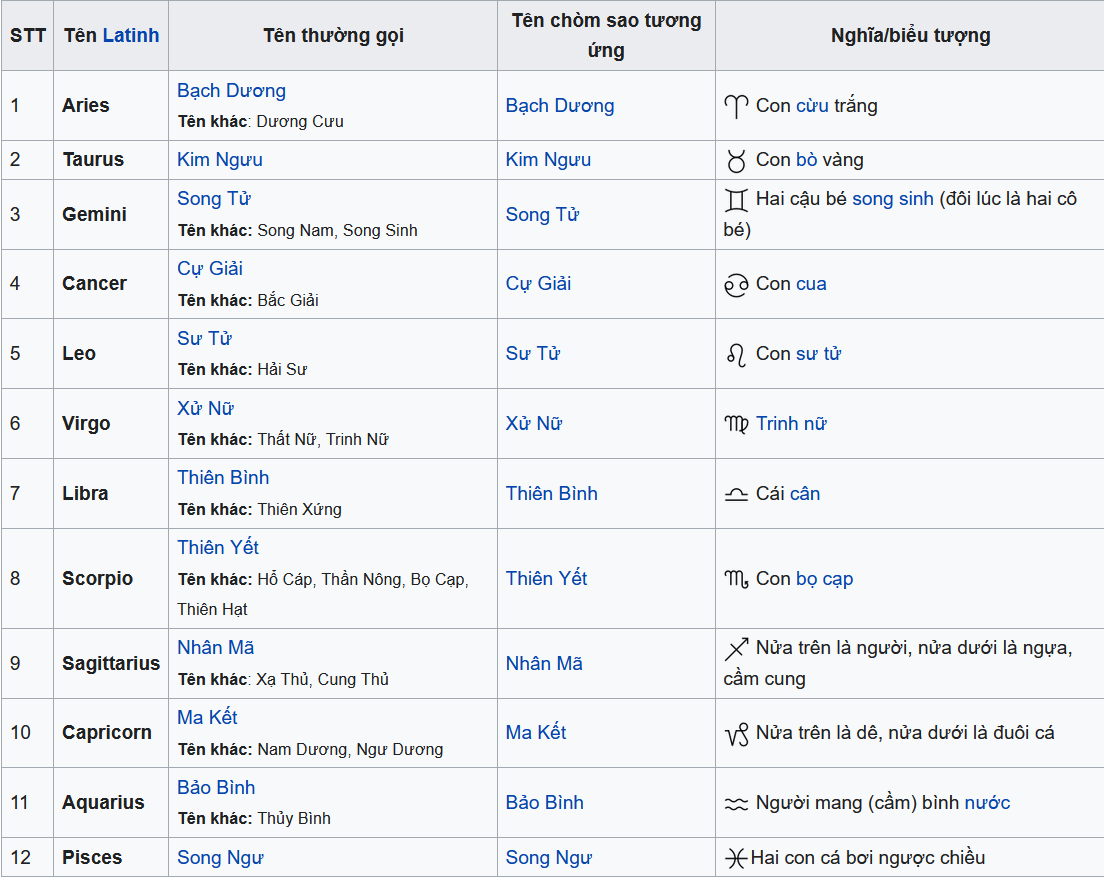
\includegraphics[scale=0.6]{../figs/G10-033-4}
%\end{center}
\section{Mục tiêu bài học - Ví dụ minh họa}
\begin{dang}{Xác định phương hướng dựa vào bầu trời sao}
	\viduii{2}{Trình bày hiểu biết của em về cách thức xác định phương hướng dựa vào bầu trời sao.
	}
	{	\begin{center}
			\textbf{Hướng dẫn trả lời}
		\end{center}
		
		Vào ban đêm, khi quan sát bầu trời, chúng ta sẽ thấy các ngôi sao sáng, tối khác nhau. Dựa vào vị trí các sao, ta có thể xác định được phương hướng và thời điểm lúc quan sát.
		\begin{itemize}
			\item Định hướng bằng sao Bắc Cực:
			
			Ở Bắc bán cầu, sao Bắc Cực có thể giúp ta tìm hướng Bắc. Sao Bắc Cực là là sao sáng nhất trong chòm Gấu Nhỏ. Tuy nhiên, đây không phải là sao sáng nhất trên bầu trời đêm. Có thể định hướng sao Bắc Cực dựa vào chòm sao Gấu Lớn hoặc chòm sao Thiên Hậu như đã đề cập ở trên.
			
			\item Định hướng bằng chòm sao Nam Thập:
			
			\begin{minipage}{0.6\textwidth}
				Ở Nam bán cầu, chòm sao Nam Thập (Nam Tào) có thể dùng để xác định hướng Nam. Chòm sao này gồm năm ngôi sao, và bốn sao sáng nhất tạo thành hình cây thập tự. Ngôi sao Hướng Nam là ngôi sao ở vị trí có đường kéo dài gấp 5 lần chiều dài cây thập tự. Hạ vuông góc ngôi sao Hướng Nam đó xuống mặt đất thì đó chính là hướng Nam trên mặt đất.
			\end{minipage}
			\begin{minipage}{0.3\textwidth}
				\begin{center}
					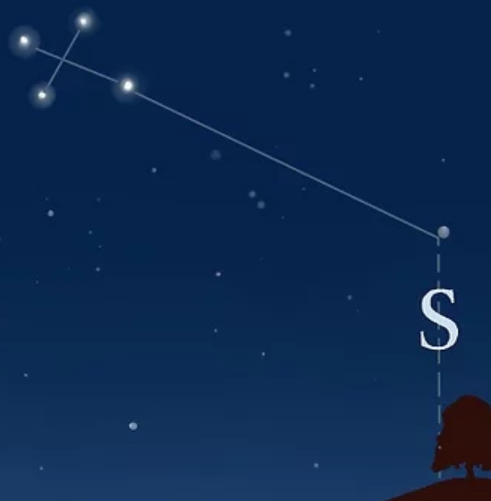
\includegraphics[scale=0.4]{../figs/G10-034-6}
				\end{center}
			\end{minipage}
			
			\item Định hướng dựa vào hướng Mặt Trời mọc và lặn:
			
			Mặt Trời mọc ở hướng Đông và lặn ở hướng Tây, do đó ta có thể dùng vị trí của Mặt Trời mọc và lặn để xác định phương hướng. Lưu ý Mặt Trời chỉ mọc đúng chính Đông hoặc lặn đúng chính Tây vào xuân phân hoặc thu phân (sẽ được trình bày ở bài sau).
		\end{itemize}
	}
	\viduii{2}{Các chòm sao thay đổi vị trí trên bầu trời như thế nào?
	}
	{	\begin{center}
			\textbf{Hướng dẫn trả lời}
		\end{center}
		
		Ở mỗi một địa điểm trên Trái Đất, khi quan sát bầu trời sao vào các mùa khác nhau, chúng ta sẽ thấy các chòm sao khác nhau.
		
		Các chòm sao luôn chuyển động trên bầu trời theo hướng từ Đông sang Tây khi ta quan sát từ Trái Đất, nhưng sao Bắc Cực ở gần phía cực Bắc của Trái Đất gần như không thay đổi vị trí.
		
	}
\end{dang}
\begin{dang}{Xác định các chòm sao trên bản đồ sao}
	\viduii{2}{Cho biết hình dạng của chòm sao Thiên Hậu, chòm sao Gấu Bé, chòm sao Gấu Lớn như hình sau. Hãy xác định vị trí của các chòm sao này trên bản đồ sao Bán Cầu Bắc.
		\begin{center}
			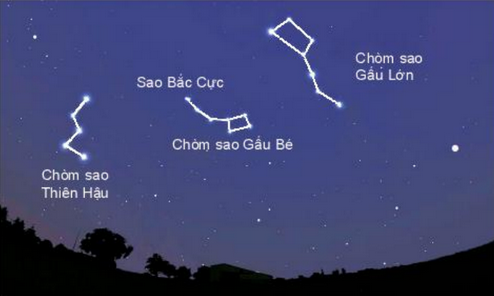
\includegraphics[scale=0.6]{../figs/G10-034-7}
		\end{center}
	}
	{	\begin{center}
			\textbf{Hướng dẫn trả lời}
		\end{center}
		
		Học sinh luyện tập nhìn bản đồ sao để xác định các chòm sao quan trọng kể trên.
		\begin{center}
			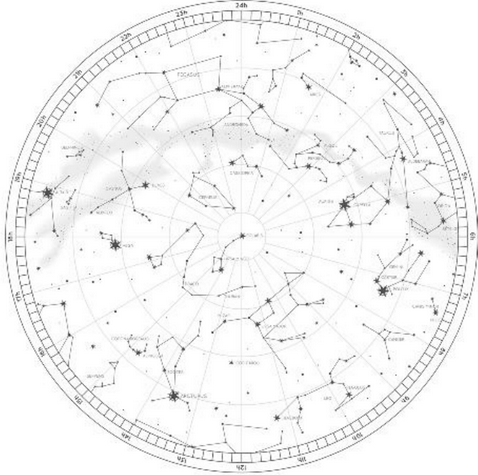
\includegraphics[scale=0.8]{../figs/G10-034-8}
		\end{center}
		
	}
	\viduii{2}{Hãy xác định hình dạng các chòm sao trong thực tế và định hướng trong không gian thông qua ứng dụng Stellarium. 
	}
	{	\begin{center}
			\textbf{Hướng dẫn trả lời}
		\end{center}
		
		Học sinh luyện tập sử dụng ứng dụng \url{https://stellarium.org} hoặc website \url{https://stellarium-web.org} để xác định các chòm sao trên bầu trời.
	}
\end{dang}
